\chapter{Implementation}

\textbf{Author: } 

\section{Generating test data}
Good test data is of utmost importance in machine learning. The system can only know information that is depicted in the training data, which is why it is important to include as many aspects of the problem as possible in this data.

Since machine learning needs a lot of data in order to solve the given task it can be tiresome to generate and label all this data by hand. Therefore the authors decided to simulate the objects and the camera using a computer graphics modelling software called Blender.

Blender allows for relatively easy generation of training data by providing a Python API. With this API almost anything that can be done using the blender user interface can also be done using Python.

For generating data the first step for the authors was to model a scene, as seen in Figure~\ref{pic:implementation_generatingData_blenderSetup}. This scene would contain a building split into multiple rooms. Each of the rooms is home to one object, which was rendered using two cameras, representing two points of view. The first camera is positioned relative to the object, whereas the second camera is positioned relative to the first camera, guaranteeing a different view on the object. Lastly, the two renders formed one input for the neural network.

%[TODO: Image camera setup, lightning, objects in Blender]
\begin{figure}[h!]
	\centering
	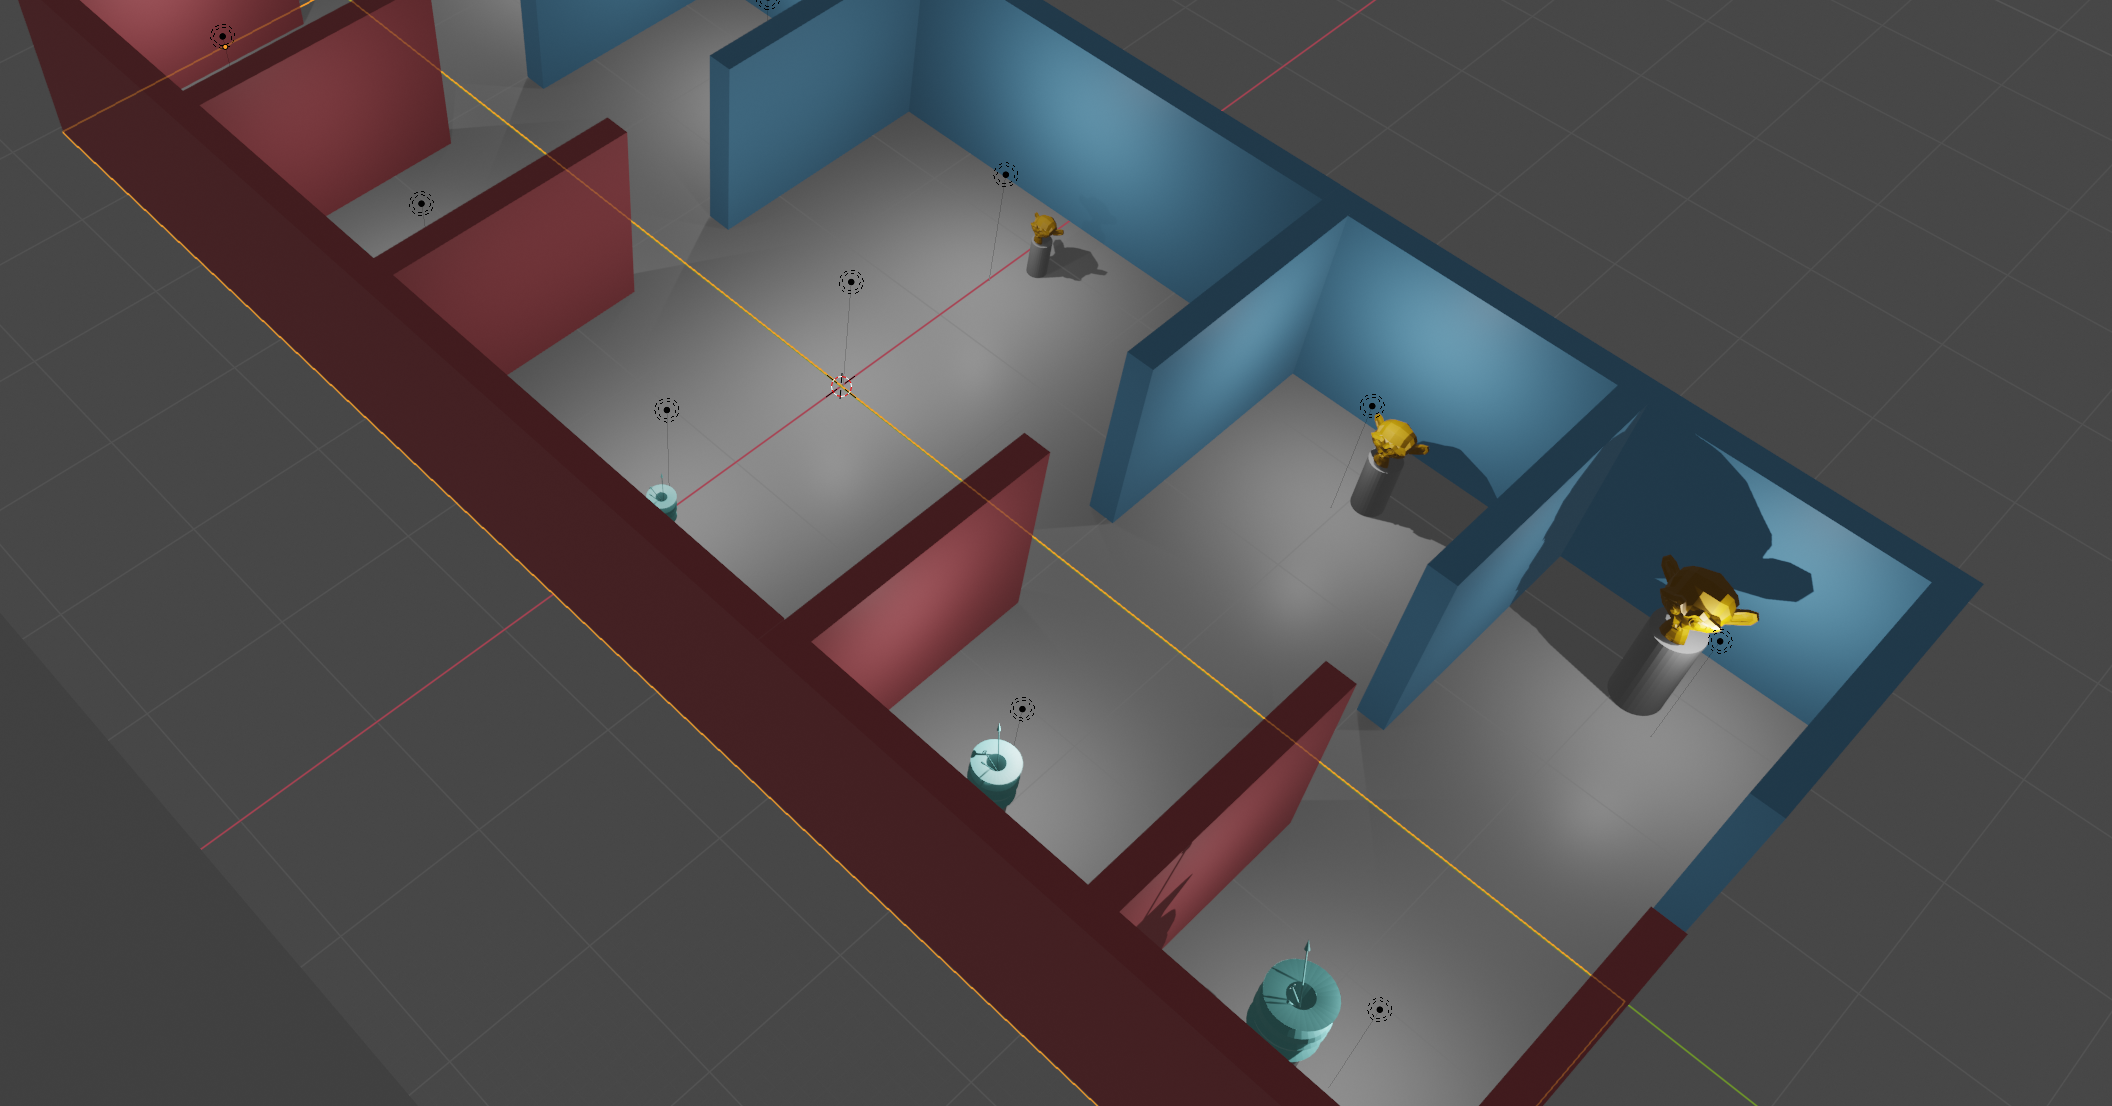
\includegraphics[width=5in]{img/implementation_generatingData_blenderSetup.png}
	\caption{The test scene for generating data. Each object is placed in a room and is separated by walls.}
	\label{pic:implementation_generatingData_blenderSetup}
\end{figure}

%[TODO: Renders and labels for example objects]
For the test objects the authors used two objects. One is a already existing monkey head in blender, the other one has been self-modelled and represents a vase with some decorating sticks in it. Both objects can be seen in Figure~\ref{pic:implementation_generatingData_testObject1} and in Figure~\ref{pic:implementation_generatingData_testObject2}.

\begin{figure}[h!]
	\centering
	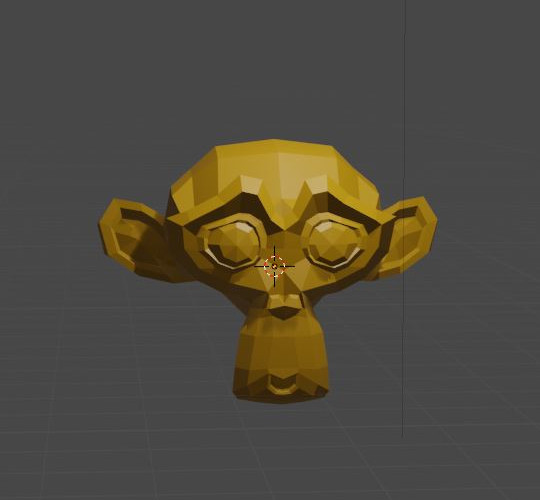
\includegraphics[width=5in]{img/implementation_generatingData_testObject1.jpg}
	\caption{One of the test objects - a monkey head.}
	\label{pic:implementation_generatingData_testObject1}
\end{figure}

\begin{figure}[h!]
	\centering
	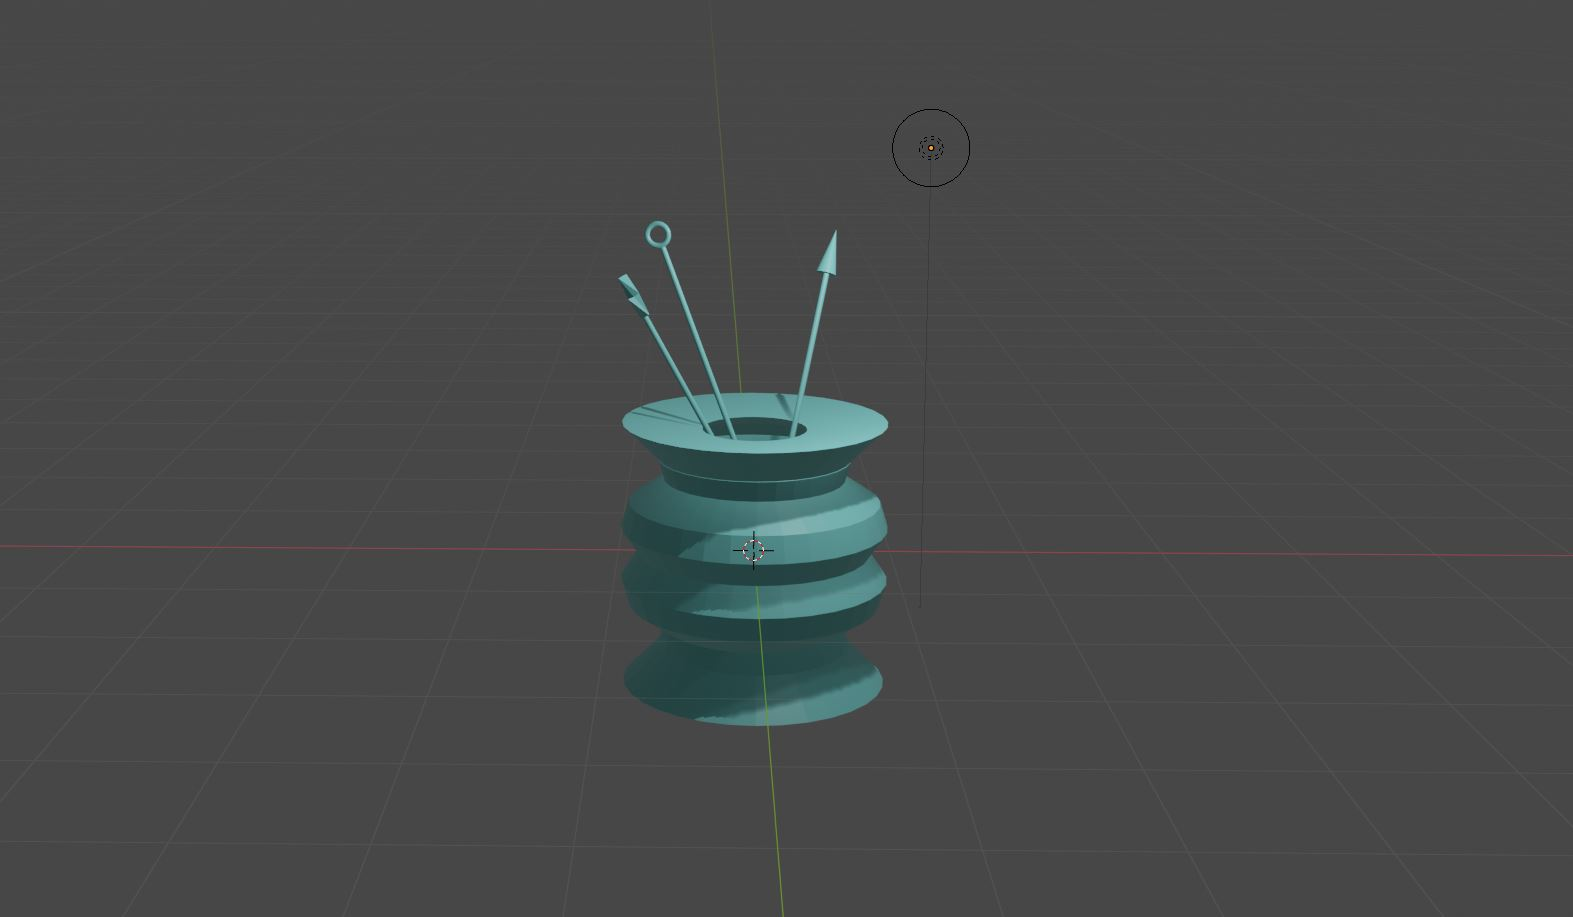
\includegraphics[width=5in]{img/implementation_generatingData_testObject2.jpg}
	\caption{One of the test objects - a decorative vase.}
	\label{pic:implementation_generatingData_testObject2}
\end{figure}

\subsection{Generating the Render-Pairs}
The following code generates the two needed renders for one of the test objects:

\begin{lstlisting}[language=python]
# Generate for 1 object
def generate_1(renderpath, infopath, target_name, iterations):
target_loc = bpy.data.objects[target_name].location

XMIN = target_loc.x - 0.6 if target_loc.x > 0 else target_loc.x + 0.6
XMAX = target_loc.x - 8.6 if target_loc.x > 0 else target_loc.x + 8.6
YMIN = target_loc.y - 1.85
YMAX = target_loc.y + 1.85
ZMIN = 0.75
ZMAX = 2

RENDERPATH = renderpath + target_name
INFOPATH = infopath + target_name

RENDERFILEPATH = RENDERPATH + "/{}-{}.jpg"
INFOFILEPATH = INFOPATH + "/{}-{}.txt"

make_dirs(RENDERPATH, INFOPATH)

for i in range(0, iterations):
# Calculate values
X = random.uniform(XMIN, XMAX)
Y1 = random.uniform(YMIN, YMAX)
Y2 = Y1 + 1 if (Y1 - target_loc.y) < 0 else Y1 - 1
Z = random.uniform(ZMIN, ZMAX)

# Add first camera
add_camera(X, Y1, Z, target_name)
write_dist_info(INFOFILEPATH, target_name, i, 1)
render(RENDERFILEPATH, i, 1)
del_cameras()

# Add second camera
add_camera(X, Y2, Z, target_name)
write_dist_info(INFOFILEPATH, target_name, i, 2)
render(RENDERFILEPATH, i, 2)
del_cameras()
\end{lstlisting}

This code can seem overwhelming at first, so the authors decided to explain each part of it. The first code block

\begin{lstlisting}[language=python]
target_loc = bpy.data.objects[target_name].location

XMIN = target_loc.x - 0.6 if target_loc.x > 0 else target_loc.x + 0.6
XMAX = target_loc.x - 8.6 if target_loc.x > 0 else target_loc.x + 8.6
YMIN = target_loc.y - 1.85
YMAX = target_loc.y + 1.85
ZMIN = 0.75
ZMAX = 2
\end{lstlisting}

stores the location of the given target, or object, in the variable 'target\_loc'. Relative to this location the min/max values for the X/Y/Z coordinates are being calculated. These coordinates are used for the camera placement, so the camera is placed relatively to the object. 'YMIN', for example means, that the camera's Y value can be no further than 1.85m to the left of the object. 'YMAX' clamps this value so there is a border on the right side as well.

\begin{lstlisting}[language=python]
# Calculate values
X = random.uniform(XMIN, XMAX)
Y1 = random.uniform(YMIN, YMAX)
Y2 = Y1 + 1 if (Y1 - target_loc.y) < 0 else Y1 - 1
Z = random.uniform(ZMIN, ZMAX)
\end{lstlisting}

This code block right here does exactly what described before. A random value for X/Y/Z is chosen. Notice that the Y value is split in two, where 'Y1' uses 'YMIN' and 'YMAX' and 'Y2' uses 'Y1' for calculation. This is to guarantee a different angle to the object, because camera one will use 'Y1' and the second camera will use 'Y2'.

[TODO: Maybe add image illustrating above text]

\begin{lstlisting}[language=python]
# Add first camera
add_camera(X, Y1, Z, target_name)
write_dist_info(INFOFILEPATH, target_name, i, 1)
render(RENDERFILEPATH, i, 1)
del_cameras()

# Add second camera
add_camera(X, Y2, Z, target_name)
write_dist_info(INFOFILEPATH, target_name, i, 2)
render(RENDERFILEPATH, i, 2)
del_cameras()
\end{lstlisting}

This last code block is basically the same for each camera. The first camera uses 'Y1' for its placement, centered on 'target\_name' (the object). Then, from the location of the first camera, the distance to the object is calculated and written to a file. After the calculation of the actual distance blender renders an image from the first camera's point of view, after which the first camera is being deleted. This is the same for the second camera, except it uses 'Y2' for its placement.

\section{OpenCV}
OpenCV is a framework for image manipulation. Some of its use cases are changing the colour spectrum, filtering the image by colour and cropping images. The authors use OpenCV to test whether there are differences between filters for the images in the training data, for example greyscale images compared to coloured images. An example render, which OpenCV gets as an input can be seen in Figure~\ref{pic:implementation_opencv_original}.

\begin{figure}[h!]
	\centering
	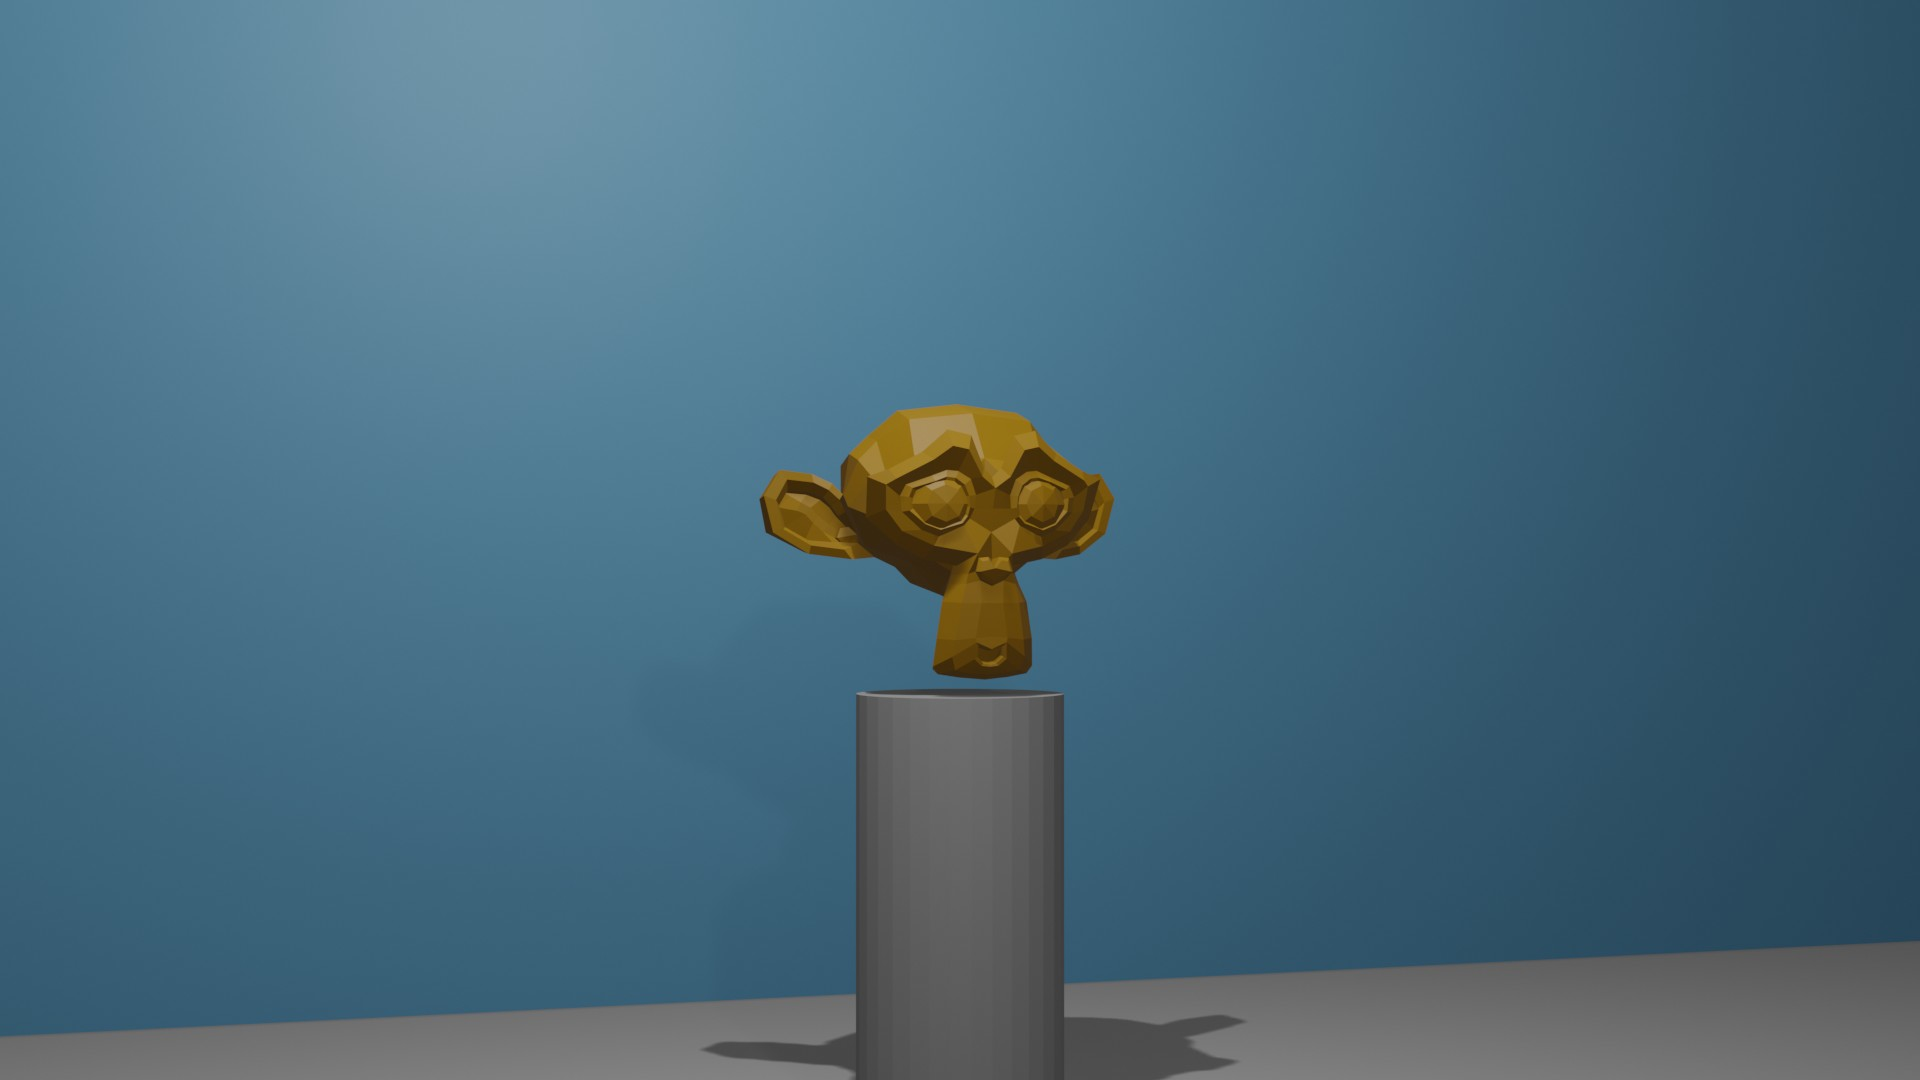
\includegraphics[width=5in]{img/implementation_opencv_original.png}
	\caption{One of two original renders produced by Blender, both depicting the same object from different points of view.}	%22_2
	\label{pic:implementation_opencv_original}
\end{figure}

\subsection{Greyscale}
Converting an image into greyscale can easily be achieved by the following OpenCV code:

\begin{lstlisting}[language=python]
import cv2

image = cv2.imread('path/to/image')
image_greyscale = cv2.cvtColor(image, cv2.COLOR_BGR2GRAY)
cv2.imwrite('path/for/saving/greyscale/image', image_greyscale)
\end{lstlisting}

This code first reads the image into 'image'. Then it converts the color of 'image' into a greyscale format and stores the result into 'image\_greyscale', which is then written to the specified path. The output generated by this code is depicted in Figure~\ref{pic:implementation_opencv_greyscale}.

\begin{figure}[h!]
	\centering
	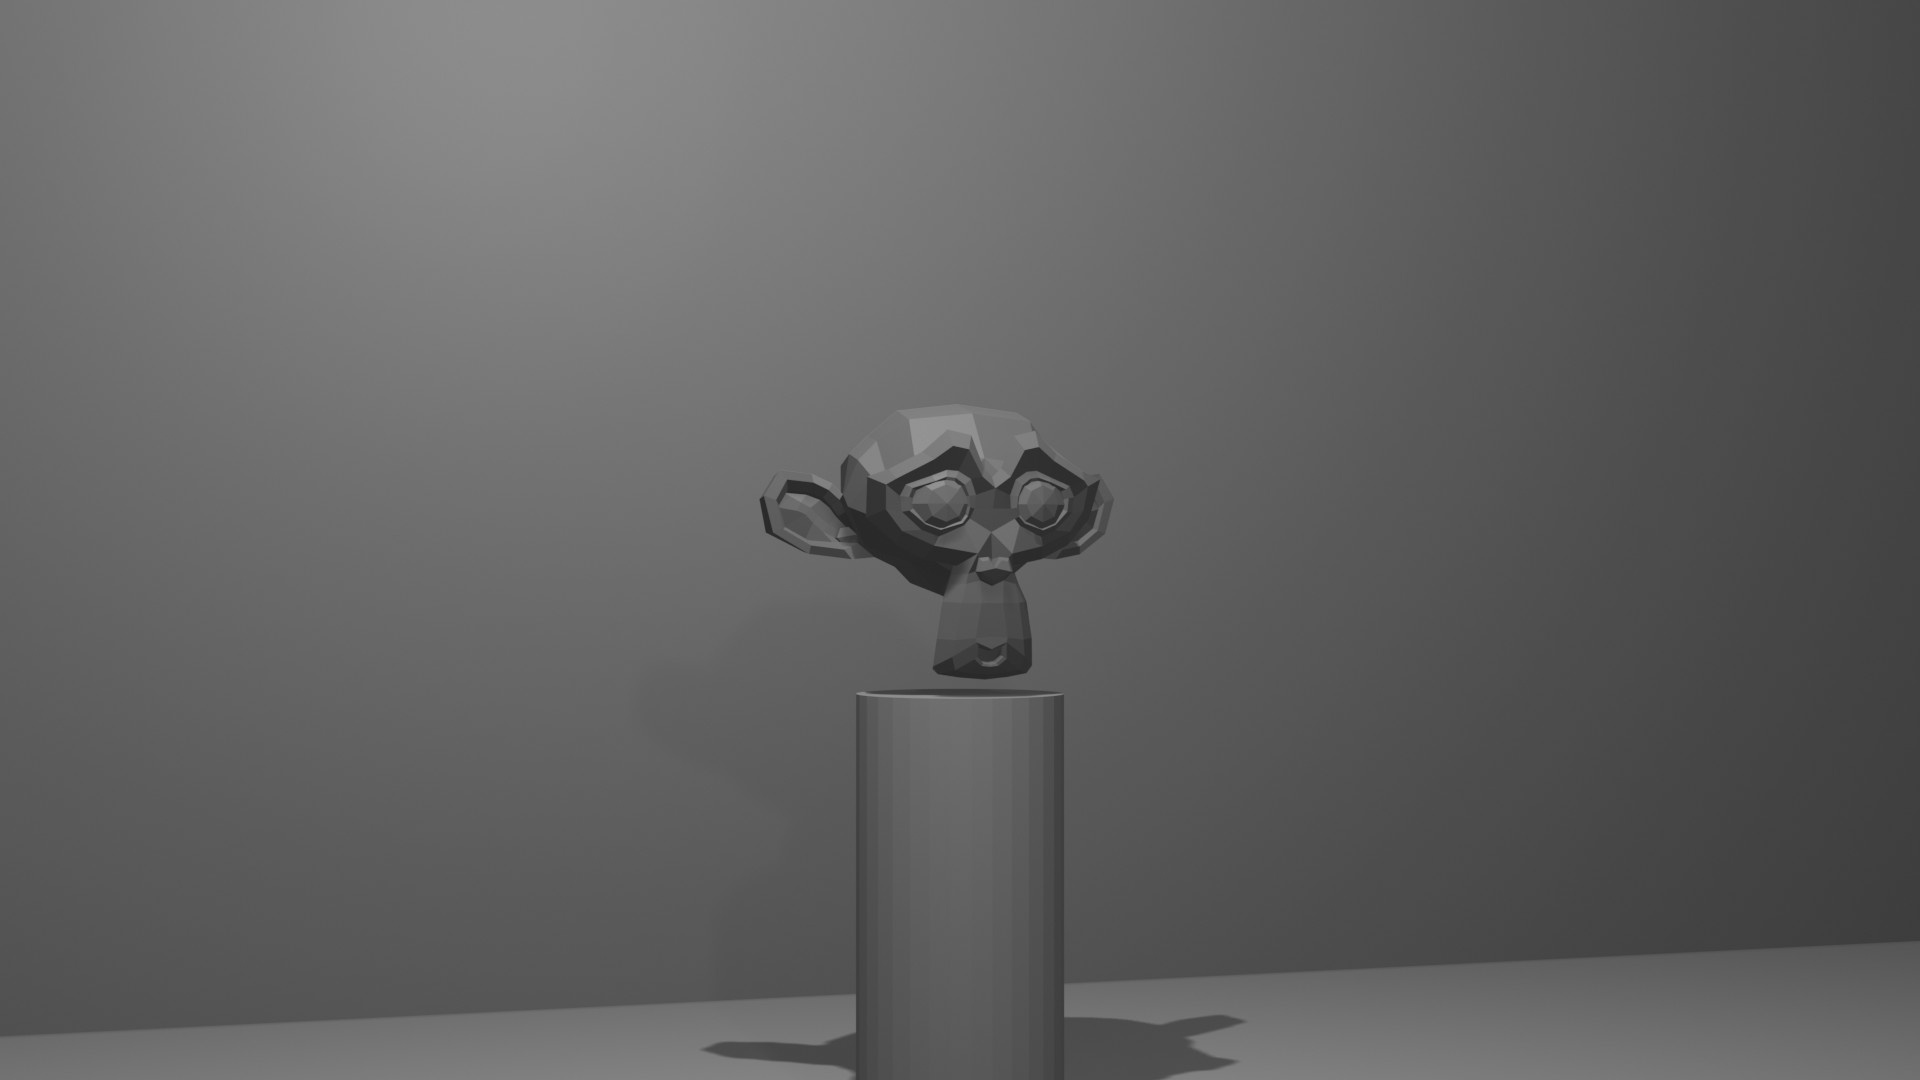
\includegraphics[width=5in]{img/implementation_opencv_greyscale.png}
	\caption{The greyscale image produced by OpenCV.}
	\label{pic:implementation_opencv_greyscale}
\end{figure}

The advantage of using greyscale images in Neural Networks is the simplification of the input layer. In greyscale images each pixel can be represented by a single decimal value between 0 and 1. This enables the first layer of the neural network to be two dimensional instead of the three dimensional counterpart, where each pixel is represented by the three decimal values for the red, green and blue colour channels.

\subsection{Resolution}
By reducing the resolution of an image the density of pixels is lessened. In this process information, that can not be regained, is lost. The OpenCV code for downscaling the images used by the authors is the following:

\begin{lstlisting}[language=python]
import cv2

image = cv2.imread('path/to/image')

scale_percent = 10  # percent of original size
width = int(image.shape[1] * scale_percent / 100)
height = int(image.shape[0] * scale_percent / 100)
dim = (width, height)

downscaled = cv2.resize(image, dim)
cv2.imwrite('{}/{}'.format(newdir_path, filename), downscaled)
\end{lstlisting}

OpenCV provides a resize function, which takes an image and the new dimensions of the image as an argument and outputs the resized image. To make sure the aspect ratio stays the same new image dimensions are calculated as a percentage of the original ones.

The output image of this code can be found in Figure~\ref{pic:implementation_opencv_resolution}.

\begin{figure}[h!]
	\centering
	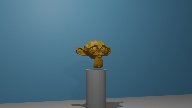
\includegraphics[width=4.5in]{img/implementation_opencv_resolution.jpg}
	\caption{Image with lower resolution than the original one. Due to the fact that the image is displayed in the same size as Figure~\ref{pic:implementation_opencv_original}, the pixel size in this image appears larger.}
	\label{pic:implementation_opencv_resolution}
\end{figure}

Downscaling the images before they are passed into the Neural Network can be profitable, because the number of weights in the first layer of the network is reduced. This can advance the learning speed.

\subsection{Cropping}
Cropping an image can remove unnecessary or unwanted parts of an image by simply cutting off areas. This is often wanted in photography to only keep what is interesting in a photo and to shift the view of the viewer to specific areas. However, the authors guess that cropping an image will worsen performance of the neural network, because information of the relative sizes are partly lost. It basically compares to zooming into the image.

Such a cropped image produced by the following code can be found in Figure~\ref{pic:implementation_opencv_cropping}.

\begin{lstlisting}[language=python]
import cv2

image = cv2.imread('path/to/image')

crop_margin_percent = 5
crop_margin_width = int(image.shape[1] * crop_margin_percent / 100)
crop_margin_height = int(image.shape[0] * crop_margin_percent / 100)

crop_img = image[crop_margin_width:-crop_margin_width, crop_margin_height:-crop_margin_height]
cv2.imwrite('{}/{}'.format(newdir_path, filename), crop_img)
\end{lstlisting}

\begin{figure}[h!]
	\centering
	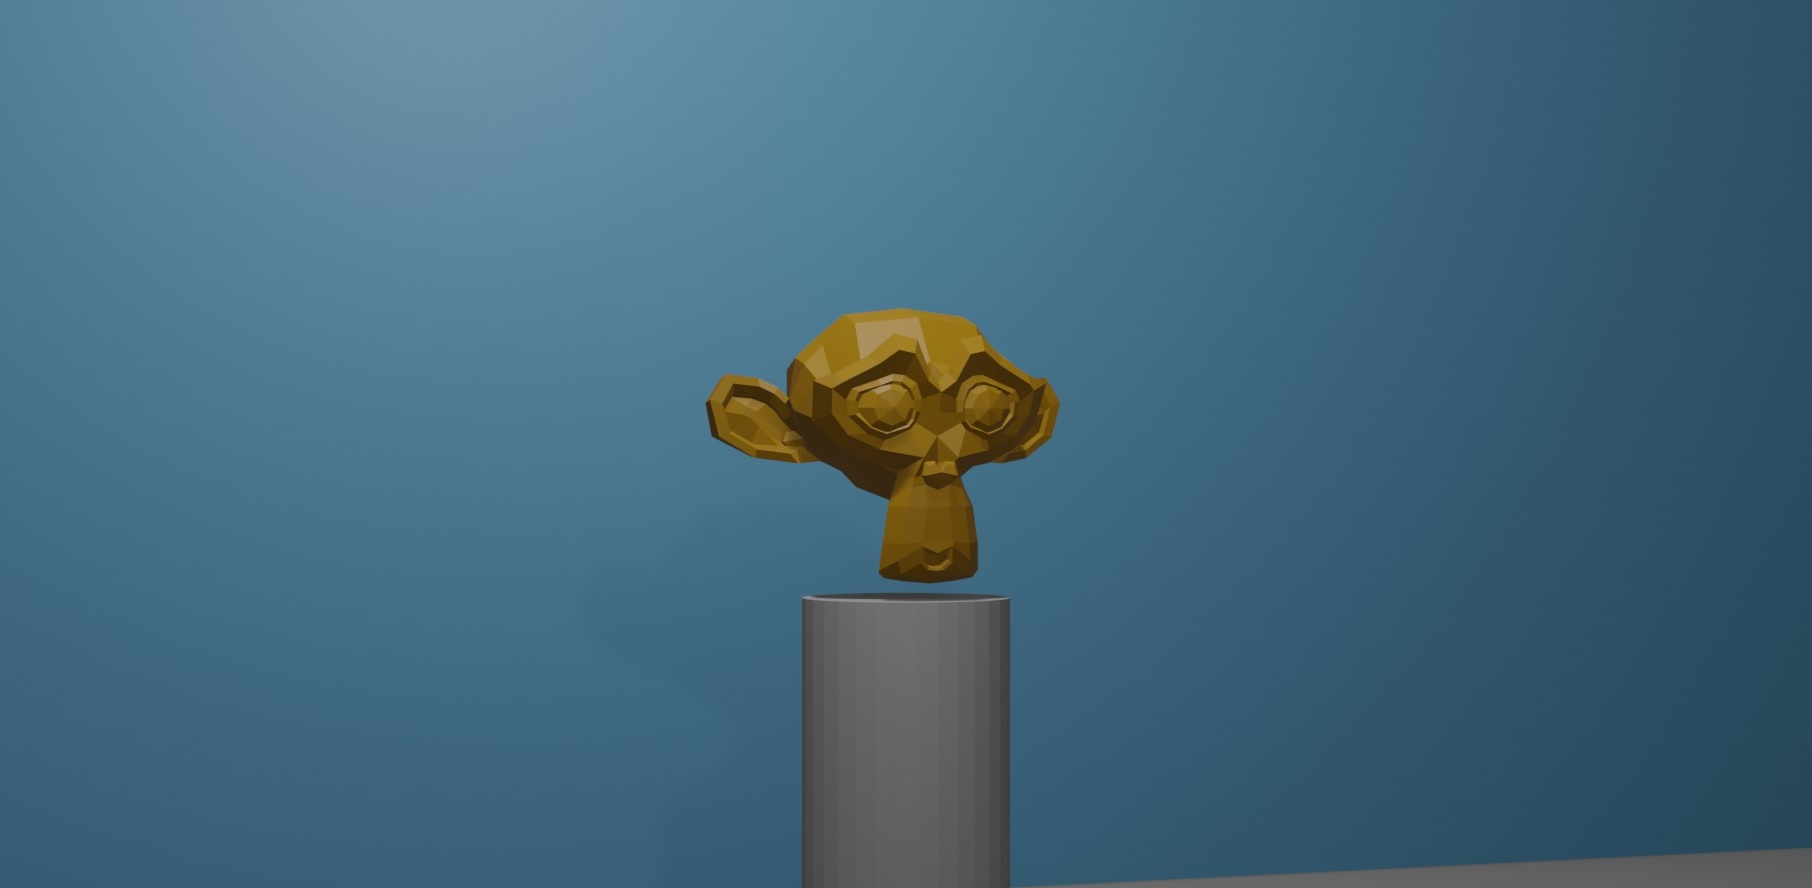
\includegraphics[width=4.5in]{img/implementation_opencv_cropping.jpg}
	\caption{In this image five percent of each side was removed, therefore the object appears closer if the image is displayed in the same size. Some information positioned in the outer areas of the image are lost during the cropping process.}
	\label{pic:implementation_opencv_cropping}
\end{figure}

\subsection{Saturated}
A saturated image means stronger colours, basically making them more distinguishable from each other. If an image is not saturated enough, colours appear as "washed out" and differences in colour are difficult to determine. Therefore, in order to help the neural network, the authors decided to also test with saturated versions of these images.

\begin{lstlisting}[language=python]
import cv2

image = cv2.imread('path/to/image')

hsv = cv2.cvtColor(image, cv2.COLOR_BGR2HSV).astype('float32')
(h, s, v) = cv2.split(hsv)
s *= 1.5
s = np.clip(s, 0, 255)
hsv = cv2.merge([h, s, v])
saturated = cv2.cvtColor(hsv.astype('uint8'), cv2.COLOR_HSV2BGR)
cv2.imwrite('{}/{}'.format(newdir_path, filename), saturated)
\end{lstlisting}

To saturate an image using OpenCV it has to be converted into the HSV colour representation. The HSV representation specifies each colour as a hue, a saturation and a value. Therefore changing the saturation in this model is relatively easy, as the saturation value of each pixel can simply be multiplied by a constant. Before the image can be converted back into the bgr colour representation the saturation values are restricted between 0 and 255, the lowest and highest saturation possible. The result achieved by this code can be seen in Figure~\ref{pic:implementation_opencv_saturated}.

\begin{figure}[h!]
	\centering
	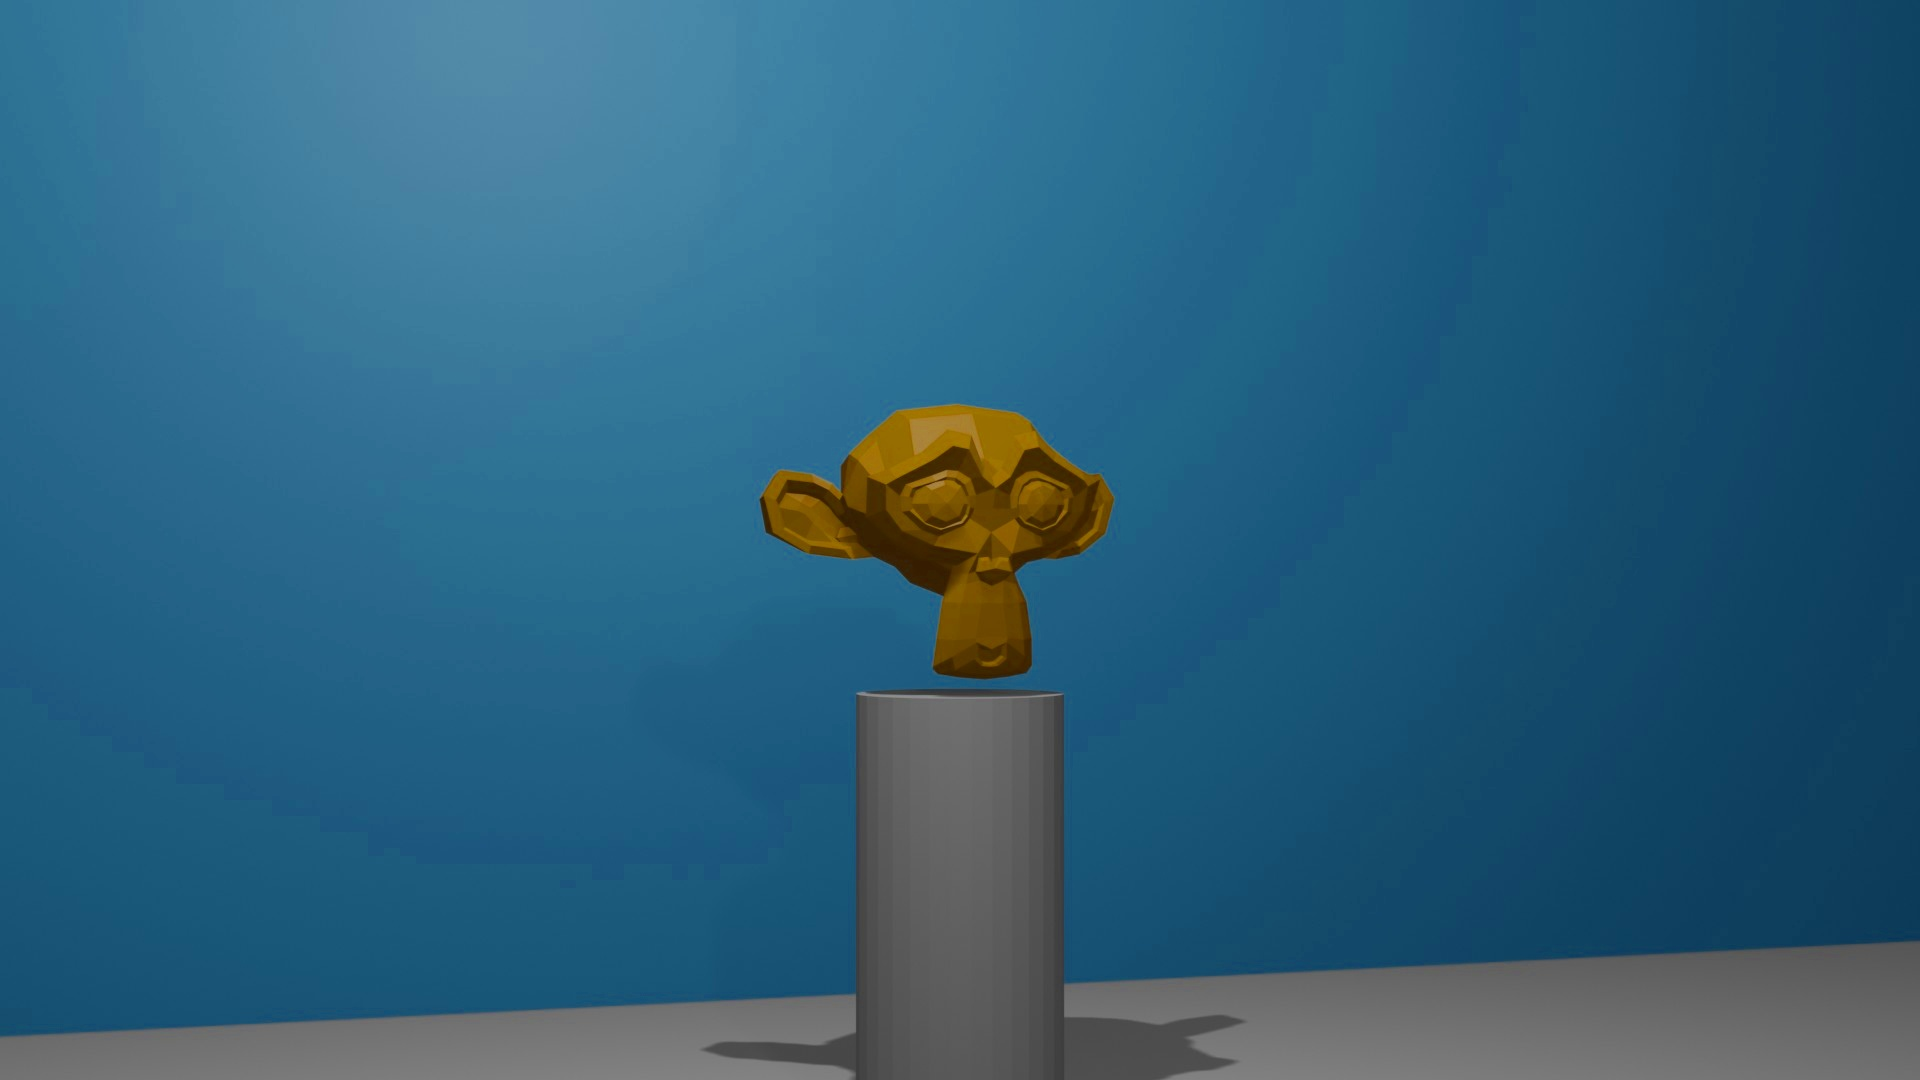
\includegraphics[width=4.5in]{img/implementation_opencv_saturated.jpg}
	\caption{Comparison between normal and saturated image.}
	\label{pic:implementation_opencv_saturated}
\end{figure}

\subsection{Brightness}
Because the neural network should also work in different environment, where other methods could have problems, the authors also tested with overly bright images. This makes it very hard to notice dark areas, such as shadows, to help with distances between objects and scaling of objects.

\begin{lstlisting}[language=python]
import cv2

image = cv2.imread('path/to/image')

alpha = 1  # contrast
beta = 60  # brightness
bright_img = cv2.convertScaleAbs(image, alpha=alpha, beta=beta)

cv2.imwrite('{}/{}'.format(newdir_path, filename), bright_img)
\end{lstlisting}

\begin{figure}[h!]
	\centering
	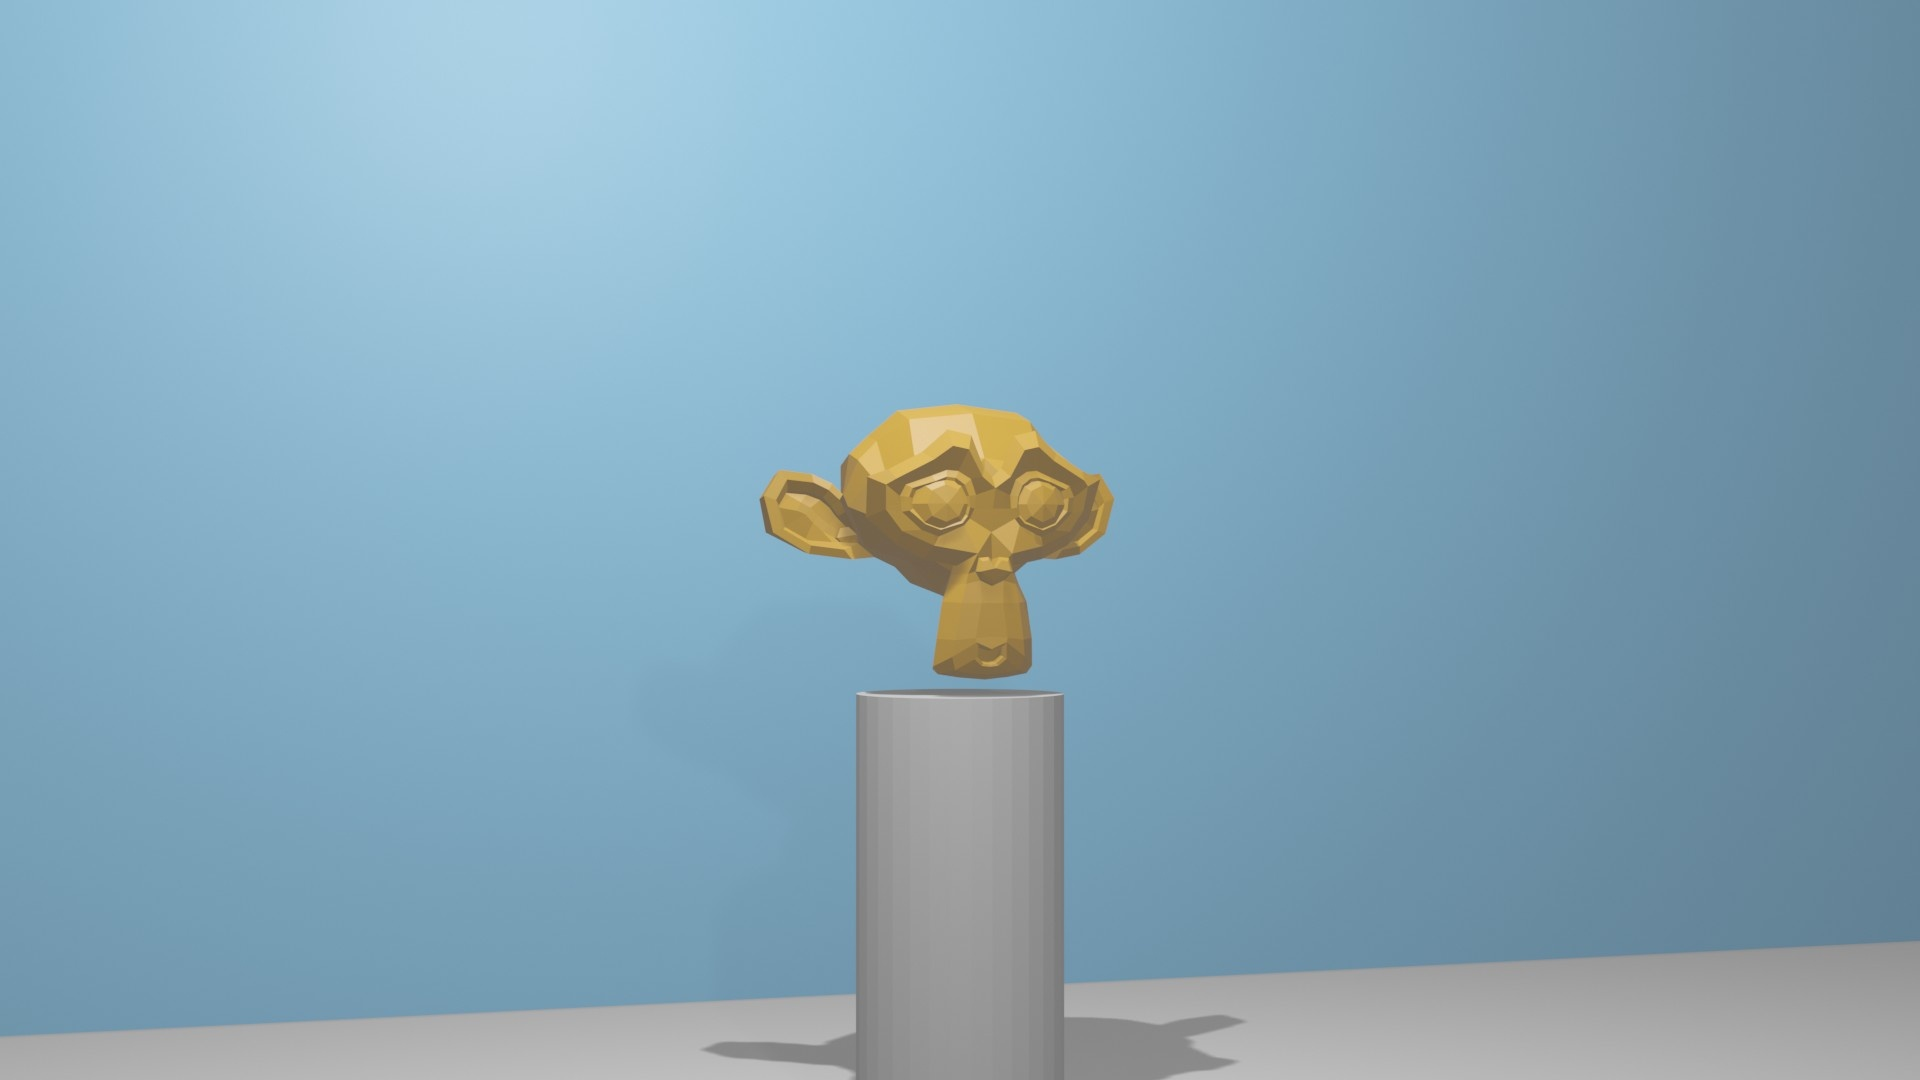
\includegraphics[width=4.5in]{img/implementation_opencv_brightness.jpg}
	\caption{The original image (Figure~\ref{pic:implementation_opencv_original}) modified by the brightening code. The image appears more washed out, as all colours are move similar due to them having moved closer to white.}
	\label{pic:implementation_opencv_brightness}
\end{figure}

\section{Neural Network}
\subsection{Testing the structure of the Neural Network}



\subsection{Structure of our Neural Network}

[wie lesen wir Daten ein, wie viele layer, was ist der output (maximale entfernung? z.B. 10m)]

\section{C++ Implementation}

\section{Technical difficulties}

\filbreak
